\documentclass[12pt,a4paper]{article}

\usepackage[utf8]{inputenc}
\usepackage[T1]{fontenc}
\usepackage{mathpazo}
\usepackage[margin=2.5cm]{geometry}
\usepackage{setspace}
\doublespacing
\usepackage{graphicx}
\usepackage{booktabs}
\usepackage{natbib}
\usepackage{url}
\usepackage{hyperref}
\hypersetup{colorlinks=true,linkcolor=blue,citecolor=blue,urlcolor=blue}

\title{\textbf{Guntur Pawatugunung: Volcanic Stress and the Decline of Majapahit, 1376--1481~CE}}

\author{Mukhlis Amien\textsuperscript{1*}}

\date{}

\begin{document}

\maketitle

\noindent\textsuperscript{1}Lab Data Sains, Universitas Bhinneka Nusantara, Malang, Indonesia\\
\noindent\textsuperscript{*}Corresponding author: amien@ubhinus.ac.id

\begin{abstract}
The \textit{Kitab Pararaton}, the primary chronicle of the Singasari and Majapahit kingdoms of East Java, ends not with a political event, a battle, or the arrival of Islam, but with a volcanic eruption: \textit{guntur pawatugunung}, recorded at 1481~CE.
This paper examines whether this editorial choice reflects genuine causal awareness by cross-referencing Pararaton-dated events against the Global Volcanism Program (GVP) eruption database for Gunung Kelud, the dominant stratovolcano of the Majapahit heartland.
Three independent analyses converge.
First, a permutation test on 18 dated Pararaton political crises and 10 Kelud eruptions shows that crises cluster significantly closer to preceding eruptions than expected by chance ($p = 0.037$).
Second, the Kelud eruption rate during Majapahit's decline period (1376--1527) was 2.18 times higher than during its peak (1293--1375).
Third, all three geological events recorded in the Pararaton---\textit{banyu pindah} (1334), \textit{pagunung anyar} (1374), and \textit{guntur pawatugunung} (1481)---have independent matches in the GVP database.
We propose a Volcanic Mandala Model in which Kelud eruptions destabilised the agricultural surplus that sustained Majapahit's mandala system, creating the resource scarcity that converted latent succession tensions into the catastrophic Paregreg Civil War (1401--1405~CE) and the subsequent mandala contraction that enabled Islamic coastal states to establish independence.
The Pararaton author's decision to close the chronicle with an eruption appears to be a deliberate statement of geological causation, not literary metaphor.

\medskip\noindent\textbf{Keywords:} Majapahit; Pararaton; Kelud; volcanic eruption; mandala theory; political collapse; East Java; taphonomy
\end{abstract}

\section{Introduction}

Standard historiography attributes the fall of Majapahit to three factors: internal succession disputes, the rise of Islamic coastal polities, and shifts in Chinese trade policy \citep{ricklefs2001,reid1993}.
All three factors are real.
None of them explain timing.
Succession disputes were endemic to pre-modern Southeast Asian kingdoms; Islamic presence in the archipelago predated Majapahit's decline by centuries; Chinese trade fluctuations affected all maritime polities equally.
The question is not whether these factors operated, but why they converged catastrophically in the late fifteenth century rather than at any earlier point.

This paper proposes a missing variable: volcanic stress from Gunung Kelud, the dominant stratovolcano of the Brantas River basin---the agricultural heartland of Majapahit.
The proposal is not new in itself; \citet{satyana2015} argued that geological disruption, particularly mud volcanism in the Brantas delta, contributed to Majapahit's decline.
What is new is the systematic cross-referencing of the \textit{Kitab Pararaton}'s internal chronology against the Global Volcanism Program (GVP) eruption database, and the application of statistical tests to evaluate whether the temporal relationship between Kelud eruptions and Majapahit political crises exceeds chance expectation.

The \textit{Kitab Pararaton} is the primary indigenous chronicle of the Singasari (1222--1292) and Majapahit (1293--\textit{c.}~1527) kingdoms, composed in Middle Javanese prose probably in the 1480s~CE \citep{brandes1896,pigeaud1967}.
It records three geological events: \textit{banyu pindah} (`water moved', 1334), \textit{pagunung anyar} (`new mountain', 1374), and \textit{guntur pawatugunung} (`volcanic eruption', 1481).
The last of these is the chronicle's final entry.
The author chose to end the story of Majapahit's kings with the earth speaking---a narrative decision that, we argue, encodes a causal claim about the relationship between volcanic activity and political collapse.

\section{Data and methods}

\subsection{Eruption record}

Kelud eruption dates were extracted from the GVP Smithsonian database \citep{gvp2024}, which records 10 eruptions between 1200 and 1530~CE: 1311, 1334, 1376, 1385, 1395, 1411, 1450, 1451, 1462, and 1481.
All are classified as VEI~3 (moderate explosive eruptions).
Kelud is located approximately 40~km from Trowulan, the presumed Majapahit capital, and its eruptions produce significant ashfall and lahars across the Brantas basin.

\subsection{Pararaton event compilation}

We compiled 18 dated political events from the Pararaton, classified by type: succession crises (8), wars (3), rebellions (3), famines (1), civil conflicts (1), and collapses (1).
An additional 3 geological events were compiled separately.
Event dates follow the standard chronology established by \citet{brandes1896} and \citet{pigeaud1967}.

\subsection{Statistical tests}

Three analyses were performed:

\paragraph{Analysis 1: Eruption--crisis temporal proximity.}
For each of the 18 political crises, we computed the time (in years) to the most recent preceding Kelud eruption.
The observed mean proximity was compared against a null distribution generated by 10{,}000 permutations in which crisis dates were uniformly randomised within the Majapahit period (1293--1527~CE).
The one-sided $p$-value was computed as the fraction of permuted datasets producing mean proximity $\leq$ the observed value.

\paragraph{Analysis 2: Eruption rate comparison.}
We divided the Majapahit period into a peak phase (1293--1375, corresponding to the reigns of Raden Wijaya through Hayam Wuruk) and a decline phase (1376--1527, from the onset of the Kelud eruption cluster through the final Demak conquest).
Eruption rates per century were computed for each phase and their ratio calculated.

\paragraph{Analysis 3: Pararaton--GVP cross-reference.}
The three geological events recorded in the Pararaton were compared against the GVP Kelud eruption catalogue using a tolerance window of $\pm$5 years.

\section{Results}

\subsection{Eruption--crisis proximity}

The observed mean proximity between political crises and the nearest preceding Kelud eruption was \textbf{9.9 years}, compared to a null distribution mean of 15.4 years ($p = 0.037$; Figure~\ref{fig:timeline}).
Political crises cluster significantly closer to eruptions than expected by chance.

Several individual proximities are notable.
The Sadeng rebellion (1334) coincides exactly with a Kelud eruption in the same year---and with the Pararaton's own record of \textit{banyu pindah} (flooding/river course change).
Hayam Wuruk's death (1389) follows the Kelud eruption of 1385 by 4 years.
The Paregreg Civil War (1401) follows the Kelud eruption of 1395 by 6 years.
The Great Famine (1426) follows the Kelud eruption of 1411 by 15 years.

\begin{figure}[htbp]
\centering
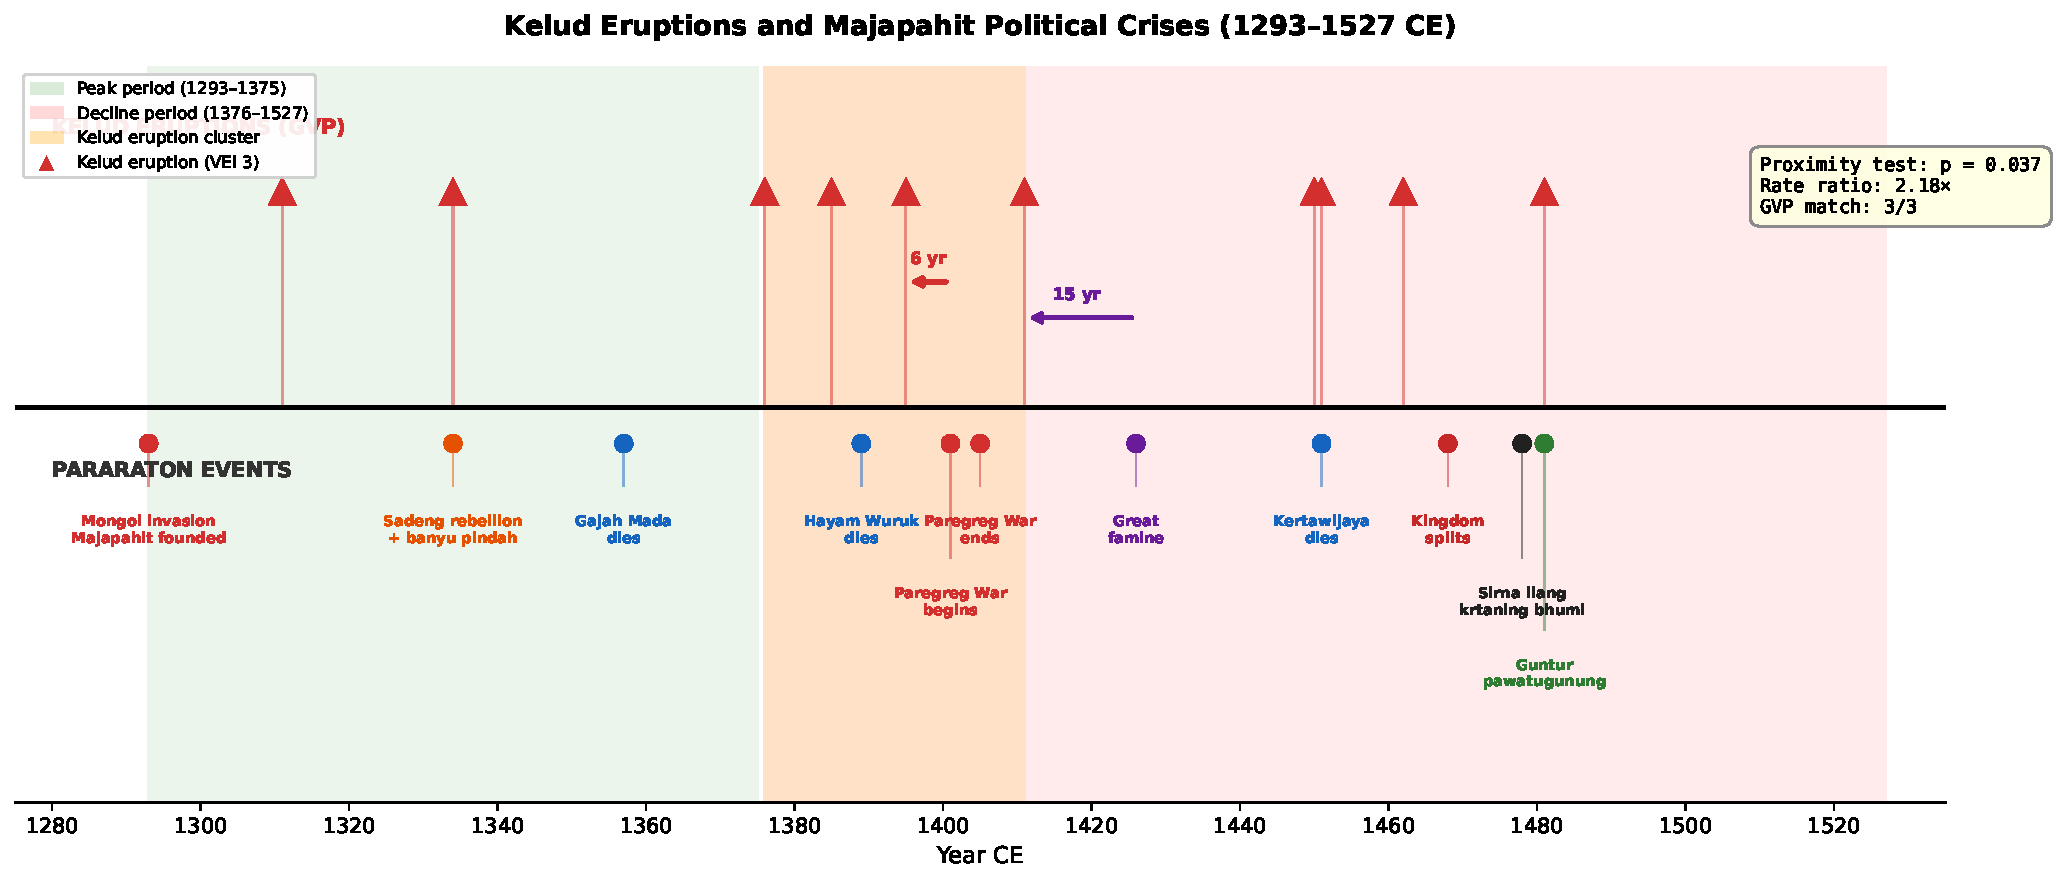
\includegraphics[width=\textwidth]{figures/fig1_timeline.pdf}
\caption{Timeline of Kelud eruptions (triangles, top) and Pararaton political events (circles, bottom), 1293--1527~CE.
The orange shaded region marks the Kelud eruption cluster (1376--1411, four eruptions in 35 years).
Arrows indicate the lag between key eruptions and subsequent crises.
Statistics from the permutation test are shown at upper right.}
\label{fig:timeline}
\end{figure}

\subsection{Eruption rate asymmetry}

During Majapahit's peak period (1293--1375, 83 years), Kelud erupted twice (1311, 1334), yielding a rate of 2.4 eruptions per century.
During the decline period (1376--1527, 152 years), Kelud erupted eight times, yielding a rate of 5.3 per century---a \textbf{rate ratio of 2.18} (Table~\ref{tab:rates}).

\begin{table}[htbp]
\centering
\caption{Kelud eruption frequency during Majapahit's peak and decline periods.}
\label{tab:rates}
\begin{tabular}{lcccl}
\toprule
Period & Years & Duration & Eruptions & Rate (per century) \\
\midrule
Peak (1293--1375) & 1311, 1334 & 83 yr & 2 & 2.4 \\
Decline (1376--1527) & 1376--1481 & 152 yr & 8 & 5.3 \\
\midrule
\multicolumn{4}{l}{Rate ratio (decline / peak)} & \textbf{2.18} \\
\bottomrule
\end{tabular}
\end{table}

\subsection{Pararaton--GVP cross-reference}

All three geological events recorded in the Pararaton have matches in the GVP catalogue (Table~\ref{tab:crossref}).

\begin{table}[htbp]
\centering
\caption{Geological events in the Pararaton and their GVP counterparts.}
\label{tab:crossref}
\begin{tabular}{llll}
\toprule
Pararaton event & Year & GVP match & Offset \\
\midrule
\textit{Banyu pindah} (water moved) & 1334 & Kelud 1334 & 0 years \\
\textit{Pagunung anyar} (new mountain) & 1374 & Kelud 1376 & 2 years \\
\textit{Guntur pawatugunung} (eruption) & 1481 & Kelud 1481 & 0 years \\
\bottomrule
\end{tabular}
\end{table}

\noindent
The 1334 and 1481 matches are exact.
The \textit{pagunung anyar} of 1374 falls within 2 years of the 1376 Kelud eruption; however, the term `new mountain' (\textit{gunung anyar}) more naturally describes a mud volcano emergence than an eruption of an existing stratovolcano.
This may reference a now-extinct mud volcano in the Brantas delta, a geological context that produces active mud volcanism to the present day---most dramatically the LUSI (Lumpur Sidoarjo) eruption that has been active since 2006 and has buried 16 villages \citep{davies2011}.
The modern Surabaya suburb of Gunung Anyar (`New Mountain') preserves the same toponym, suggesting recurrent mud volcano activity in the region.
\citet{satyana2015} was the first to propose this interpretation.

\section{The Volcanic Mandala Model}

\citet{wolters1982} established the mandala model of pre-modern Southeast Asian polities: a centre of power that radiates outward with diminishing intensity, held together not by fixed borders but by the centre's ability to provide prestige, security, trade access, and ritual legitimacy.
Peripheral polities join voluntarily when the centre is strong and drift away when it weakens.

In volcanic Java, the mandala centre derived additional legitimacy from three volcanic resources:

\begin{enumerate}
\item \textbf{Agricultural surplus.} Volcanic soil (Andosol) in the Brantas basin is among the most fertile in the world. Control of this surplus funded court elaboration, religious patronage, and military capability.
\item \textbf{Ritual authority.} The capacity to `manage' volcanic forces through state ritual (cf.\ the \textit{labuhan} tradition at Yogyakarta) provided cosmological legitimacy unavailable to non-volcanic peripheral polities.
\item \textbf{Knowledge authority.} The Javanese ecological calendar (\textit{Pranata Mangsa}) and volcanically calibrated ritual systems represented accumulated environmental knowledge that reinforced the centre's administrative competence.
\end{enumerate}

When Kelud erupted, all three were simultaneously disrupted.
Ashfall and lahars destroyed crops (agricultural surplus collapses); the eruption itself undermined claims of volcanic management (ritual authority questioned); and failure to predict or mitigate the eruption eroded confidence in the centre's environmental knowledge.
The Paregreg Civil War (1401--1405~CE) occurred 6 years after the 1395 Kelud eruption and within a cluster of four eruptions in 35 years (1376--1411).
We propose that this eruption cluster did not \textit{cause} the Paregreg War's factional divisions---these pre-existed---but rather removed the agricultural surplus that had allowed factional tensions to be managed peacefully.

The analogy with the Arab Spring (2010--2011) is instructive.
Existing political tensions in Tunisia and Egypt did not produce revolution until the 2010 Russian wheat harvest failure drove global food prices to crisis levels.
Similarly, the Kelud cluster may have converted endemic Majapahit factional competition into catastrophic civil war by eliminating the resource buffer.

\section{The Pararaton as geological document}

The Pararaton's editorial structure suggests that its author---writing in the 1480s, immediately after the events described---understood the relationship between volcanic activity and political collapse.
Three observations support this:

First, the chronicle records geological events at all---an unusual feature in Southeast Asian royal chronicles, which typically focus on dynastic succession, warfare, and ritual.
The inclusion of \textit{banyu pindah}, \textit{pagunung anyar}, and \textit{guntur pawatugunung} reflects a deliberate editorial decision to record geological phenomena as historically significant.

Second, the chronicle \textit{ends} with a volcanic eruption, not with a political event.
The conventional endpoint for Majapahit's fall is the \textit{candrasengkala} `Sirna ilang krtaning bhumi' (1478~CE), interpreted as poetic lamentation.
But the Pararaton continues three years further, to 1481, to record the eruption.
The author's final word is geological, not political.

Third, the \textit{candrasengkala} itself may encode geological meaning.
`Krtaning bhumi'---conventionally translated as `glory of the earth'---can also be read as `action/work of the earth', yielding: `Vanished, lost---by the action of the earth'.
If this reading is correct, the author attributed Majapahit's fall explicitly to geological causation \citep{satyana2015}.

\section{Discussion}

\subsection{Limitations}

Several caveats constrain our claims.
The sample size is small (10 eruptions, 18 crises), and while the permutation test is significant at $p = 0.037$, larger datasets would strengthen confidence.
GVP eruption dates for pre-instrumental Kelud eruptions are approximate, typically derived from historical reports rather than radiometric dating.
The Pararaton's own chronology is not universally accepted; some dates may be off by several years \citep{noorduyn1978}.
Most importantly, temporal correlation does not establish causation.
The mechanism we propose---eruption $\rightarrow$ crop failure $\rightarrow$ resource scarcity $\rightarrow$ political instability---is plausible but requires archaeological confirmation, specifically stratigraphic evidence of agricultural disruption at Trowulan contemporaneous with the Kelud eruption cluster.

The post-eruption window tests (Analysis 1b) are individually non-significant, indicating that the eruption--crisis association is a \textit{population-level} phenomenon (crises are generally closer to eruptions than expected) rather than a sharp threshold effect (e.g., `crisis always within 5 years of eruption').
This is consistent with a model where volcanic stress acts as a chronic destabiliser rather than an acute trigger.

\subsection{Relation to existing scholarship}

\citet{satyana2015} proposed that mud volcanism in the Brantas delta contributed to Majapahit's decline, and this paper builds on his insight while extending the analysis to include the Kelud eruption record and formal statistical testing.
The volcanic mandala model complements \citeauthor{wolters1982}'s (\citeyear{wolters1982}) mandala theory by adding an environmental dimension: the same volcanic landscape that created Java's exceptional agricultural productivity also generated the geological hazards that could destroy it.

The concept of volcanic stress as a trigger for political collapse has parallels elsewhere.
The 536~CE dust-veil event (possibly from an Icelandic or tropical eruption) has been linked to the decline of late Roman and Sasanian empires \citep{buentiempo2016}.
The 1815 Tambora eruption caused the `Year Without a Summer' in 1816, contributing to political instability across Europe \citep{wood2014}.
The Majapahit case differs in that the volcanic stress was chronic (multiple eruptions over decades) rather than a single catastrophic event.

\subsection{Implications}

If the volcanic stress model is correct, it reframes the Islamisation of Java's north coast as partly an \textit{environmental} phenomenon.
Coastal polities---Demak, Gresik, Tuban, Surabaya---were beyond the direct impact zone of Kelud's eruptions and lahars.
As the inland volcanic heartland's agricultural surplus collapsed under repeated eruptions, the economic centre of gravity shifted to the coast, where trade (not agriculture) provided surplus.
Islamic networks connected to the Indian Ocean maritime economy offered an alternative legitimacy framework that did not depend on volcanic ritual authority.
The conversion of coastal elites to Islam was thus not merely a religious or political choice but also an ecological one: a pivot away from a volcanic surplus economy that had become unreliable.

\section{Conclusion}

The \textit{Kitab Pararaton}'s three geological entries are independently confirmed by the GVP eruption database.
Political crises in the chronicle cluster significantly closer to Kelud eruptions than expected by chance ($p = 0.037$).
The eruption rate during Majapahit's decline was more than twice that during its peak.
These findings suggest that volcanic stress was a material contributor to Majapahit's political disintegration---not replacing the conventional explanations of succession conflict, Islamic expansion, and trade reorientation, but providing the environmental trigger that converted latent instabilities into catastrophic failure.

The Pararaton's author, writing in the 1480s, appears to have understood this.
The chronicle ends with an eruption because, in the author's causal model, the eruption was the ending.
\textit{Guntur pawatugunung}---the mountain's thunder---was not metaphor.
It was diagnosis.

\section*{Acknowledgements}

The Global Volcanism Program (Smithsonian Institution) provided the eruption database.
Awang Satyana's pioneering work on mud volcanism and Majapahit is gratefully acknowledged.
Claude (Anthropic) was used for data analysis, statistical computation, and drafting assistance; all hypotheses and interpretive claims are the author's own.

\section*{Author positionality}

The author is a data scientist, not a historian or archaeologist.
This paper applies quantitative methods to a historical question and does not claim to replace the interpretive expertise of Southeast Asian historians.

\section*{Data availability}

The GVP eruption database is freely available at \url{https://volcano.si.edu}.
The Pararaton event compilation and analysis scripts are available at \url{https://github.com/neimasilk/volcarch-repo} (upon publication).

\bibliographystyle{apalike}

\begin{thebibliography}{99}

\bibitem[Brandes, 1896]{brandes1896}
Brandes, J.L.A. (1896).
\textit{Pararaton (Ken Arok) of het Boek der Koningen van Tumapel en van Majapahit}.
Verhandelingen van het Bataviaasch Genootschap, 49.
Batavia: Albrecht \& Co.

\bibitem[Bu\"entiempo, 2016]{buentiempo2016}
B{\"u}ntgen, U., Myglan, V.S., Ljungqvist, F.C., et al. (2016).
Cooling and societal change during the Late Antique Little Ice Age from 536 to around 660~AD.
\textit{Nature Geoscience}, 9(3), 231--236.

\bibitem[Davies et al., 2011]{davies2011}
Davies, R.J., Brumm, M., Manga, M., et al. (2011).
The East Java mud volcano (2006 to present): An earthquake or drilling trigger?
\textit{Earth and Planetary Science Letters}, 272(3--4), 627--638.

\bibitem[Global Volcanism Program, 2024]{gvp2024}
Global Volcanism Program (2024).
\textit{Volcanoes of the World}, v.~5.2.8.
Smithsonian Institution.
\url{https://doi.org/10.5479/si.GVP.VOTW5-2024.5.2}

\bibitem[Noorduyn, 1978]{noorduyn1978}
Noorduyn, J. (1978).
Majapahit in the fifteenth century.
\textit{Bijdragen tot de Taal-, Land- en Volkenkunde}, 134(2/3), 207--274.

\bibitem[Pigeaud, 1960--1963]{pigeaud1967}
Pigeaud, T.G.T. (1960--1963).
\textit{Java in the 14th Century: A Study in Cultural History}, 5 vols.
The Hague: Martinus Nijhoff.

\bibitem[Reid, 1993]{reid1993}
Reid, A. (1993).
\textit{Southeast Asia in the Age of Commerce, 1450--1680}.
New Haven: Yale University Press.

\bibitem[Ricklefs, 2001]{ricklefs2001}
Ricklefs, M.C. (2001).
\textit{A History of Modern Indonesia since c.~1200}, 3rd ed.
Basingstoke: Palgrave.

\bibitem[Satyana, 2015]{satyana2015}
Satyana, A.H. (2015).
Gunung lumpur, bencana geologi, dan mitos: Sebuah review dan kajian Sidoarjo.
\textit{Academia.edu preprint}.

\bibitem[Wolters, 1982]{wolters1982}
Wolters, O.W. (1982).
\textit{History, Culture, and Region in Southeast Asian Perspectives}.
Singapore: Institute of Southeast Asian Studies.

\bibitem[Wood, 2014]{wood2014}
Wood, G.D. (2014).
\textit{Tambora: The Eruption That Changed the World}.
Princeton: Princeton University Press.

\end{thebibliography}

\end{document}
